\documentclass[10pt,a4paper,twocolumn]{article}
\usepackage{endfloat}
\usepackage{f1000_styles}
\usepackage{listings}
\usepackage{units}
\usepackage[colorlinks]{hyperref}
\usepackage{url}
\usepackage{appendix}
\usepackage{soul}

\definecolor{dkgreen}{rgb}{0,0.6,0}
\definecolor{gray}{rgb}{0.5,0.5,0.5}
\definecolor{mauve}{rgb}{0.58,0,0.82}

\begin{document}

\newcommand{\AVTotalRaters}{9}
\newcommand{\AVAggThresh}{50\%}
\newcommand{\AVFracWithLabeledChar}{100.0\%}
% AV total character labels
% ['ABBIEHOFFMAN', 'BOBHOPE', 'BOY', 'BUBBA', 'BUBBASGRGRANDMA', 'BUBBASGRGRGRANDMA', 'BUBBASYOUNGBROTHER', 'CHILDREN', 'CROWD', 'DAN', 'DICKCAVETT', 'ELVISPRESLEY', 'FORREST', 'FORRESTJR', 'FORRESTVO', 'GIRL', 'JENNY', 'JENNYSDAD', 'JENNYSGRANDMA', 'JOHNLENNON', 'MAN', 'MEN', 'MRSBLUE', 'MRSGUMP', 'OLDERBOYS', 'OLDMAN', 'OLDMEN', 'OLDWOMAN', 'PRESIDENTJOHNSON', 'PRESIDENTKENNEDY', 'PRESIDENTNIXON', 'ROBERTKENNEDY', 'WOMAN', 'WOMEN']
\newcommand{\AVTotalCharLabels}{34}
% AV character labels AGG > 0.50
% [('BUBBA', 231, 15), ('CROWD', 247, 14), ('DAN', 681, 29), ('FORREST', 3014, 143), ('FORRESTVO', 421, 56), ('JENNY', 1429, 55), ('MAN', 461, 46), ('MRSGUMP', 198, 20), ('WOMAN', 88, 12)]
\newcommand{\AVThreshCharLabels}{9}
\newcommand{\AVFracWithLabeledEmotions}{68.4\%}
% AV emotion labels AGG > 0.50
% [('ADMIRATION', 65, 10), ('ANGERRAGE', 430, 25), ('COMPASSION', 24, 3), ('CONTEMPT', 81, 12), ('DISAPPOINTMENT', 64, 6), ('FEAR', 612, 20), ('GLOATING', 37, 4), ('GRATITUDE', 8, 1), ('HAPPINESS', 546, 46), ('HAPPYFOR', 5, 1), ('HATE', 19, 2), ('HOPE', 6, 1), ('LOVE', 258, 28), ('PRIDE', 43, 7), ('RELIEF', 6, 1), ('REMORSE', 29, 2), ('SADNESS', 623, 30), ('SHAME', 20, 1)]
\newcommand{\AVThreshEmoLabels}{18}
\newcommand{\AVFracWithLabeledOncue}{100.0\%}
% AV oncue labels AGG > 0.50
% [('AUDIO', 267, 20), ('CONTEXT', 841, 47), ('FACE', 3481, 178), ('GESTURE', 1917, 100), ('VERBAL', 2900, 195)]
\newcommand{\AVThreshOncueLabels}{5}
\newcommand{\AVFracWithLabeledOffcue}{99.7\%}
% AV offcue labels AGG > 0.50
% [('CHARLEFT', 683, 70), ('EMOCHANGE', 1568, 59), ('EMOFADED', 725, 63), ('SCENEEND', 1741, 124)]
\newcommand{\AVThreshOffcueLabels}{4}
\newcommand{\AVCorrArousalValenceAllChar}{-0.210 $\pm$0.022}
\newcommand{\AVCorrValenceDirectionAllChar}{0.023 $\pm$0.023}
\newcommand{\AVCorrArousalDirectionAllChar}{-0.244 $\pm$0.022}
\newcommand{\AVInterRaterConsistArousalAllChar}{\textbf{0.676} $\pm$0.006}
\newcommand{\AVInterRaterConsistValenceAllChar}{\textbf{0.851} $\pm$0.004}
\newcommand{\AVInterRaterConsistDirectionAllChar}{\textbf{0.555} $\pm$0.011}
\newcommand{\AVInterRaterConsistADMIRATIONAllChar}{0.392 $\pm$0.006}
\newcommand{\AVInterRaterConsistANGERRAGEAllChar}{\textbf{0.719} $\pm$0.005}
\newcommand{\AVInterRaterConsistCOMPASSIONAllChar}{0.337 $\pm$0.010}
\newcommand{\AVInterRaterConsistCONTEMPTAllChar}{0.433 $\pm$0.008}
\newcommand{\AVInterRaterConsistDISAPPOINTMENTAllChar}{0.408 $\pm$0.008}
\newcommand{\AVInterRaterConsistFEARAllChar}{\textbf{0.749} $\pm$0.003}
\newcommand{\AVInterRaterConsistFEARSCONFIRMEDAllChar}{0.048 $\pm$0.009}
\newcommand{\AVInterRaterConsistGLOATINGAllChar}{\textbf{0.644} $\pm$0.014}
\newcommand{\AVInterRaterConsistGRATIFICATIONAllChar}{0.155 $\pm$0.010}
\newcommand{\AVInterRaterConsistGRATITUDEAllChar}{0.317 $\pm$0.012}
\newcommand{\AVInterRaterConsistHAPPINESSAllChar}{\textbf{0.618} $\pm$0.006}
\newcommand{\AVInterRaterConsistHAPPYFORAllChar}{0.478 $\pm$0.013}
\newcommand{\AVInterRaterConsistHATEAllChar}{0.441 $\pm$0.011}
\newcommand{\AVInterRaterConsistHOPEAllChar}{0.333 $\pm$0.010}
\newcommand{\AVInterRaterConsistLOVEAllChar}{\textbf{0.568} $\pm$0.008}
\newcommand{\AVInterRaterConsistPRIDEAllChar}{0.473 $\pm$0.011}
\newcommand{\AVInterRaterConsistRELIEFAllChar}{0.353 $\pm$0.019}
\newcommand{\AVInterRaterConsistREMORSEAllChar}{\textbf{0.557} $\pm$0.022}
\newcommand{\AVInterRaterConsistRESENTMENTAllChar}{n/a}
\newcommand{\AVInterRaterConsistSADNESSAllChar}{\textbf{0.737} $\pm$0.005}
\newcommand{\AVInterRaterConsistSATISFACTIONAllChar}{0.112 $\pm$0.007}
\newcommand{\AVInterRaterConsistSHAMEAllChar}{0.316 $\pm$0.006}
\newcommand{\AVInterRaterConsistAUDIOAllChar}{0.418 $\pm$0.008}
\newcommand{\AVInterRaterConsistCONTEXTAllChar}{0.384 $\pm$0.010}
\newcommand{\AVInterRaterConsistFACEAllChar}{\textbf{0.713} $\pm$0.006}
\newcommand{\AVInterRaterConsistGESTUREAllChar}{\textbf{0.619} $\pm$0.010}
\newcommand{\AVInterRaterConsistNARRATORAllChar}{n/a}
\newcommand{\AVInterRaterConsistVERBALAllChar}{\textbf{0.637} $\pm$0.008}
\newcommand{\AVCorrArousalValenceForrest}{-0.132 $\pm$0.023}
\newcommand{\AVCorrValenceDirectionForrest}{-0.031 $\pm$0.023}
\newcommand{\AVCorrArousalDirectionForrest}{-0.239 $\pm$0.022}
\newcommand{\AVInterRaterConsistArousalForrest}{\textbf{0.600} $\pm$0.008}
\newcommand{\AVInterRaterConsistValenceForrest}{\textbf{0.784} $\pm$0.006}
\newcommand{\AVInterRaterConsistDirectionForrest}{\textbf{0.543} $\pm$0.012}
\newcommand{\AVInterRaterConsistADMIRATIONForrest}{0.306 $\pm$0.015}
\newcommand{\AVInterRaterConsistANGERRAGEForrest}{\textbf{0.693} $\pm$0.006}
\newcommand{\AVInterRaterConsistCOMPASSIONForrest}{0.232 $\pm$0.019}
\newcommand{\AVInterRaterConsistCONTEMPTForrest}{n/a}
\newcommand{\AVInterRaterConsistDISAPPOINTMENTForrest}{0.431 $\pm$0.007}
\newcommand{\AVInterRaterConsistFEARForrest}{\textbf{0.729} $\pm$0.004}
\newcommand{\AVInterRaterConsistFEARSCONFIRMEDForrest}{n/a}
\newcommand{\AVInterRaterConsistGLOATINGForrest}{n/a}
\newcommand{\AVInterRaterConsistGRATIFICATIONForrest}{0.242 $\pm$0.017}
\newcommand{\AVInterRaterConsistGRATITUDEForrest}{0.267 $\pm$0.024}
\newcommand{\AVInterRaterConsistHAPPINESSForrest}{\textbf{0.561} $\pm$0.007}
\newcommand{\AVInterRaterConsistHAPPYFORForrest}{0.408 $\pm$0.028}
\newcommand{\AVInterRaterConsistHATEForrest}{0.478 $\pm$0.027}
\newcommand{\AVInterRaterConsistHOPEForrest}{0.202 $\pm$0.008}
\newcommand{\AVInterRaterConsistLOVEForrest}{0.472 $\pm$0.008}
\newcommand{\AVInterRaterConsistPRIDEForrest}{\textbf{0.536} $\pm$0.009}
\newcommand{\AVInterRaterConsistRELIEFForrest}{\textbf{0.505} $\pm$0.028}
\newcommand{\AVInterRaterConsistREMORSEForrest}{n/a}
\newcommand{\AVInterRaterConsistRESENTMENTForrest}{n/a}
\newcommand{\AVInterRaterConsistSADNESSForrest}{\textbf{0.750} $\pm$0.005}
\newcommand{\AVInterRaterConsistSATISFACTIONForrest}{n/a}
\newcommand{\AVInterRaterConsistSHAMEForrest}{0.290 $\pm$0.006}
\newcommand{\AVInterRaterConsistAUDIOForrest}{0.354 $\pm$0.013}
\newcommand{\AVInterRaterConsistCONTEXTForrest}{0.424 $\pm$0.011}
\newcommand{\AVInterRaterConsistFACEForrest}{\textbf{0.687} $\pm$0.010}
\newcommand{\AVInterRaterConsistGESTUREForrest}{\textbf{0.532} $\pm$0.011}
\newcommand{\AVInterRaterConsistNARRATORForrest}{n/a}
\newcommand{\AVInterRaterConsistVERBALForrest}{\textbf{0.565} $\pm$0.007}
\newcommand{\AVCorrArousalValenceJenny}{-0.207 $\pm$0.022}
\newcommand{\AVCorrValenceDirectionJenny}{-0.248 $\pm$0.022}
\newcommand{\AVCorrArousalDirectionJenny}{0.099 $\pm$0.023}
\newcommand{\AVInterRaterConsistArousalJenny}{\textbf{0.688} $\pm$0.006}
\newcommand{\AVInterRaterConsistValenceJenny}{\textbf{0.858} $\pm$0.003}
\newcommand{\AVInterRaterConsistDirectionJenny}{\textbf{0.576} $\pm$0.012}
\newcommand{\AVInterRaterConsistADMIRATIONJenny}{n/a}
\newcommand{\AVInterRaterConsistANGERRAGEJenny}{\textbf{0.809} $\pm$0.007}
\newcommand{\AVInterRaterConsistCOMPASSIONJenny}{0.459 $\pm$0.018}
\newcommand{\AVInterRaterConsistCONTEMPTJenny}{0.404 $\pm$0.020}
\newcommand{\AVInterRaterConsistDISAPPOINTMENTJenny}{n/a}
\newcommand{\AVInterRaterConsistFEARJenny}{\textbf{0.633} $\pm$0.005}
\newcommand{\AVInterRaterConsistFEARSCONFIRMEDJenny}{n/a}
\newcommand{\AVInterRaterConsistGLOATINGJenny}{n/a}
\newcommand{\AVInterRaterConsistGRATIFICATIONJenny}{n/a}
\newcommand{\AVInterRaterConsistGRATITUDEJenny}{0.165 $\pm$0.015}
\newcommand{\AVInterRaterConsistHAPPINESSJenny}{\textbf{0.738} $\pm$0.005}
\newcommand{\AVInterRaterConsistHAPPYFORJenny}{n/a}
\newcommand{\AVInterRaterConsistHATEJenny}{n/a}
\newcommand{\AVInterRaterConsistHOPEJenny}{0.439 $\pm$0.026}
\newcommand{\AVInterRaterConsistLOVEJenny}{\textbf{0.660} $\pm$0.009}
\newcommand{\AVInterRaterConsistPRIDEJenny}{n/a}
\newcommand{\AVInterRaterConsistRELIEFJenny}{n/a}
\newcommand{\AVInterRaterConsistREMORSEJenny}{0.464 $\pm$0.006}
\newcommand{\AVInterRaterConsistRESENTMENTJenny}{n/a}
\newcommand{\AVInterRaterConsistSADNESSJenny}{\textbf{0.695} $\pm$0.009}
\newcommand{\AVInterRaterConsistSATISFACTIONJenny}{n/a}
\newcommand{\AVInterRaterConsistSHAMEJenny}{0.201 $\pm$0.015}
\newcommand{\AVInterRaterConsistAUDIOJenny}{0.203 $\pm$0.007}
\newcommand{\AVInterRaterConsistCONTEXTJenny}{\textbf{0.547} $\pm$0.010}
\newcommand{\AVInterRaterConsistFACEJenny}{\textbf{0.880} $\pm$0.004}
\newcommand{\AVInterRaterConsistGESTUREJenny}{\textbf{0.769} $\pm$0.009}
\newcommand{\AVInterRaterConsistNARRATORJenny}{n/a}
\newcommand{\AVInterRaterConsistVERBALJenny}{\textbf{0.783} $\pm$0.005}
\newcommand{\AOTotalRaters}{3}
\newcommand{\AOAggThresh}{50\%}
\newcommand{\AOFracWithLabeledChar}{100.0\%}
% AO total character labels
% ['ABBIEHOFFMAN', 'BARBERSHOP', 'BOY', 'BUBBA', 'CROWD', 'DAN', 'DICKCAVETT', 'ELVISPRESLEY', 'FORREST', 'FORRESTJR', 'FORRESTVO', 'GIRL', 'GUY', 'IN', 'JENNY', 'JENNYSDAD', 'JOHNLENNON', 'MAN', 'MEN', 'MRSBLUE', 'MRSGUMP', 'NARRATOR', 'NEILARMSTRONG', 'OLDERBOYS', 'OLDMAN', 'OLDWOMAN', 'PRESIDENTJOHNSON', 'PRESIDENTKENNEDY', 'PRESIDENTNIXON', 'WOMAN']
\newcommand{\AOTotalCharLabels}{30}
% AO character labels AGG > 0.50
% [('BOY', 16, 9), ('DAN', 816, 19), ('FORREST', 1960, 58), ('FORRESTVO', 210, 23), ('JENNY', 1023, 32), ('MAN', 711, 36), ('MRSGUMP', 108, 9), ('WOMAN', 73, 6)]
\newcommand{\AOThreshCharLabels}{8}
\newcommand{\AOFracWithLabeledEmotions}{97.5\%}
% AO emotion labels AGG > 0.50
% [('ADMIRATION', 151, 12), ('ANGERRAGE', 400, 27), ('COMPASSION', 27, 3), ('CONTEMPT', 63, 9), ('DISAPPOINTMENT', 54, 6), ('FEAR', 616, 12), ('GLOATING', 2, 1), ('GRATITUDE', 21, 1), ('HAPPINESS', 893, 54), ('HATE', 49, 3), ('HOPE', 36, 2), ('LOVE', 375, 19), ('PRIDE', 30, 5), ('REMORSE', 32, 2), ('SADNESS', 583, 25), ('SHAME', 41, 4)]
\newcommand{\AOThreshEmoLabels}{16}
\newcommand{\AOFracWithLabeledOncue}{100.0\%}
% AO oncue labels AGG > 0.50
% [('AUDIO', 133, 8), ('CONTEXT', 102, 6), ('NARRATOR', 203, 15), ('VERBAL', 2965, 140)]
\newcommand{\AOThreshOncueLabels}{4}
\newcommand{\AOFracWithLabeledOffcue}{98.1\%}
% AO offcue labels AGG > 0.50
% [('CHARLEFT', 98, 22), ('EMOCHANGE', 1260, 35), ('EMOFADED', 27, 7), ('SCENEEND', 2171, 121)]
\newcommand{\AOThreshOffcueLabels}{4}
\newcommand{\AOCorrArousalValenceAllChar}{-0.087 $\pm$0.023}
\newcommand{\AOCorrValenceDirectionAllChar}{0.061 $\pm$0.023}
\newcommand{\AOCorrArousalDirectionAllChar}{-0.039 $\pm$0.023}
\newcommand{\AOInterRaterConsistArousalAllChar}{0.305 $\pm$0.078}
\newcommand{\AOInterRaterConsistValenceAllChar}{\textbf{0.564} $\pm$0.044}
\newcommand{\AOInterRaterConsistDirectionAllChar}{0.068 $\pm$0.050}
\newcommand{\AOInterRaterConsistADMIRATIONAllChar}{0.343 $\pm$0.094}
\newcommand{\AOInterRaterConsistANGERRAGEAllChar}{0.377 $\pm$0.042}
\newcommand{\AOInterRaterConsistCOMPASSIONAllChar}{0.182 $\pm$0.013}
\newcommand{\AOInterRaterConsistCONTEMPTAllChar}{0.157 $\pm$0.043}
\newcommand{\AOInterRaterConsistDISAPPOINTMENTAllChar}{0.367 $\pm$0.095}
\newcommand{\AOInterRaterConsistFEARAllChar}{\textbf{0.546} $\pm$0.108}
\newcommand{\AOInterRaterConsistFEARSCONFIRMEDAllChar}{n/a}
\newcommand{\AOInterRaterConsistGLOATINGAllChar}{0.045 $\pm$0.038}
\newcommand{\AOInterRaterConsistGRATIFICATIONAllChar}{n/a}
\newcommand{\AOInterRaterConsistGRATITUDEAllChar}{n/a}
\newcommand{\AOInterRaterConsistHAPPINESSAllChar}{0.289 $\pm$0.107}
\newcommand{\AOInterRaterConsistHAPPYFORAllChar}{n/a}
\newcommand{\AOInterRaterConsistHATEAllChar}{0.097 $\pm$0.070}
\newcommand{\AOInterRaterConsistHOPEAllChar}{0.217 $\pm$0.060}
\newcommand{\AOInterRaterConsistLOVEAllChar}{0.396 $\pm$0.032}
\newcommand{\AOInterRaterConsistPRIDEAllChar}{0.156 $\pm$0.054}
\newcommand{\AOInterRaterConsistRELIEFAllChar}{-0.003 $\pm$0.001}
\newcommand{\AOInterRaterConsistREMORSEAllChar}{0.323 $\pm$0.107}
\newcommand{\AOInterRaterConsistRESENTMENTAllChar}{n/a}
\newcommand{\AOInterRaterConsistSADNESSAllChar}{0.464 $\pm$0.023}
\newcommand{\AOInterRaterConsistSATISFACTIONAllChar}{n/a}
\newcommand{\AOInterRaterConsistSHAMEAllChar}{0.185 $\pm$0.112}
\newcommand{\AOInterRaterConsistAUDIOAllChar}{0.037 $\pm$0.051}
\newcommand{\AOInterRaterConsistCONTEXTAllChar}{n/a}
\newcommand{\AOInterRaterConsistFACEAllChar}{n/a}
\newcommand{\AOInterRaterConsistGESTUREAllChar}{n/a}
\newcommand{\AOInterRaterConsistNARRATORAllChar}{0.251 $\pm$0.047}
\newcommand{\AOInterRaterConsistVERBALAllChar}{0.368 $\pm$0.107}
\newcommand{\AOCorrArousalValenceForrest}{-0.027 $\pm$0.023}
\newcommand{\AOCorrValenceDirectionForrest}{0.089 $\pm$0.023}
\newcommand{\AOCorrArousalDirectionForrest}{0.178 $\pm$0.022}
\newcommand{\AOInterRaterConsistArousalForrest}{0.443 $\pm$0.078}
\newcommand{\AOInterRaterConsistValenceForrest}{0.440 $\pm$0.054}
\newcommand{\AOInterRaterConsistDirectionForrest}{-0.059 $\pm$0.072}
\newcommand{\AOInterRaterConsistADMIRATIONForrest}{n/a}
\newcommand{\AOInterRaterConsistANGERRAGEForrest}{0.141 $\pm$0.100}
\newcommand{\AOInterRaterConsistCOMPASSIONForrest}{n/a}
\newcommand{\AOInterRaterConsistCONTEMPTForrest}{n/a}
\newcommand{\AOInterRaterConsistDISAPPOINTMENTForrest}{0.456 $\pm$0.129}
\newcommand{\AOInterRaterConsistFEARForrest}{\textbf{0.504} $\pm$0.072}
\newcommand{\AOInterRaterConsistFEARSCONFIRMEDForrest}{n/a}
\newcommand{\AOInterRaterConsistGLOATINGForrest}{n/a}
\newcommand{\AOInterRaterConsistGRATIFICATIONForrest}{n/a}
\newcommand{\AOInterRaterConsistGRATITUDEForrest}{n/a}
\newcommand{\AOInterRaterConsistHAPPINESSForrest}{0.381 $\pm$0.060}
\newcommand{\AOInterRaterConsistHAPPYFORForrest}{n/a}
\newcommand{\AOInterRaterConsistHATEForrest}{n/a}
\newcommand{\AOInterRaterConsistHOPEForrest}{n/a}
\newcommand{\AOInterRaterConsistLOVEForrest}{0.327 $\pm$0.092}
\newcommand{\AOInterRaterConsistPRIDEForrest}{n/a}
\newcommand{\AOInterRaterConsistRELIEFForrest}{n/a}
\newcommand{\AOInterRaterConsistREMORSEForrest}{0.453 $\pm$0.364}
\newcommand{\AOInterRaterConsistRESENTMENTForrest}{n/a}
\newcommand{\AOInterRaterConsistSADNESSForrest}{\textbf{0.522} $\pm$0.006}
\newcommand{\AOInterRaterConsistSATISFACTIONForrest}{n/a}
\newcommand{\AOInterRaterConsistSHAMEForrest}{0.034 $\pm$0.036}
\newcommand{\AOInterRaterConsistAUDIOForrest}{n/a}
\newcommand{\AOInterRaterConsistCONTEXTForrest}{n/a}
\newcommand{\AOInterRaterConsistFACEForrest}{n/a}
\newcommand{\AOInterRaterConsistGESTUREForrest}{n/a}
\newcommand{\AOInterRaterConsistNARRATORForrest}{0.202 $\pm$0.045}
\newcommand{\AOInterRaterConsistVERBALForrest}{0.455 $\pm$0.042}
\newcommand{\AOCorrArousalValenceJenny}{-0.207 $\pm$0.022}
\newcommand{\AOCorrValenceDirectionJenny}{-0.332 $\pm$0.021}
\newcommand{\AOCorrArousalDirectionJenny}{0.029 $\pm$0.023}
\newcommand{\AOInterRaterConsistArousalJenny}{0.330 $\pm$0.076}
\newcommand{\AOInterRaterConsistValenceJenny}{\textbf{0.598} $\pm$0.079}
\newcommand{\AOInterRaterConsistDirectionJenny}{0.053 $\pm$0.145}
\newcommand{\AOInterRaterConsistADMIRATIONJenny}{\textbf{0.643} $\pm$0.197}
\newcommand{\AOInterRaterConsistANGERRAGEJenny}{\textbf{0.626} $\pm$0.109}
\newcommand{\AOInterRaterConsistCOMPASSIONJenny}{0.363 $\pm$0.042}
\newcommand{\AOInterRaterConsistCONTEMPTJenny}{n/a}
\newcommand{\AOInterRaterConsistDISAPPOINTMENTJenny}{n/a}
\newcommand{\AOInterRaterConsistFEARJenny}{0.392 $\pm$0.013}
\newcommand{\AOInterRaterConsistFEARSCONFIRMEDJenny}{n/a}
\newcommand{\AOInterRaterConsistGLOATINGJenny}{n/a}
\newcommand{\AOInterRaterConsistGRATIFICATIONJenny}{n/a}
\newcommand{\AOInterRaterConsistGRATITUDEJenny}{n/a}
\newcommand{\AOInterRaterConsistHAPPINESSJenny}{\textbf{0.532} $\pm$0.108}
\newcommand{\AOInterRaterConsistHAPPYFORJenny}{n/a}
\newcommand{\AOInterRaterConsistHATEJenny}{n/a}
\newcommand{\AOInterRaterConsistHOPEJenny}{\textbf{0.804} $\pm$0.052}
\newcommand{\AOInterRaterConsistLOVEJenny}{0.432 $\pm$0.040}
\newcommand{\AOInterRaterConsistPRIDEJenny}{n/a}
\newcommand{\AOInterRaterConsistRELIEFJenny}{n/a}
\newcommand{\AOInterRaterConsistREMORSEJenny}{n/a}
\newcommand{\AOInterRaterConsistRESENTMENTJenny}{n/a}
\newcommand{\AOInterRaterConsistSADNESSJenny}{0.228 $\pm$0.040}
\newcommand{\AOInterRaterConsistSATISFACTIONJenny}{n/a}
\newcommand{\AOInterRaterConsistSHAMEJenny}{n/a}
\newcommand{\AOInterRaterConsistAUDIOJenny}{n/a}
\newcommand{\AOInterRaterConsistCONTEXTJenny}{n/a}
\newcommand{\AOInterRaterConsistFACEJenny}{n/a}
\newcommand{\AOInterRaterConsistGESTUREJenny}{n/a}
\newcommand{\AOInterRaterConsistNARRATORJenny}{\textbf{0.578} $\pm$0.286}
\newcommand{\AOInterRaterConsistVERBALJenny}{\textbf{0.626} $\pm$0.168}
\newcommand{\InterModCorrArousalAllChar}{0.474 $\pm$0.018}
\newcommand{\InterModCorrValenceAllChar}{\textbf{0.726} $\pm$0.011}
\newcommand{\InterModCorrDirectionAllChar}{0.425 $\pm$0.019}
\newcommand{\InterModCorrADMIRATIONAllChar}{0.260 $\pm$0.022}
\newcommand{\InterModCorrANGERRAGEAllChar}{0.485 $\pm$0.018}
\newcommand{\InterModCorrCOMPASSIONAllChar}{0.232 $\pm$0.022}
\newcommand{\InterModCorrCONTEMPTAllChar}{0.201 $\pm$0.022}
\newcommand{\InterModCorrDISAPPOINTMENTAllChar}{0.372 $\pm$0.020}
\newcommand{\InterModCorrFEARAllChar}{\textbf{0.673} $\pm$0.013}
\newcommand{\InterModCorrFEARSCONFIRMEDAllChar}{n/a}
\newcommand{\InterModCorrGLOATINGAllChar}{0.231 $\pm$0.022}
\newcommand{\InterModCorrGRATIFICATIONAllChar}{0.062 $\pm$0.023}
\newcommand{\InterModCorrGRATITUDEAllChar}{0.201 $\pm$0.022}
\newcommand{\InterModCorrHAPPINESSAllChar}{\textbf{0.532} $\pm$0.016}
\newcommand{\InterModCorrHAPPYFORAllChar}{0.289 $\pm$0.021}
\newcommand{\InterModCorrHATEAllChar}{0.266 $\pm$0.022}
\newcommand{\InterModCorrHOPEAllChar}{0.181 $\pm$0.022}
\newcommand{\InterModCorrLOVEAllChar}{\textbf{0.618} $\pm$0.014}
\newcommand{\InterModCorrPRIDEAllChar}{0.203 $\pm$0.022}
\newcommand{\InterModCorrRELIEFAllChar}{0.062 $\pm$0.023}
\newcommand{\InterModCorrREMORSEAllChar}{0.376 $\pm$0.020}
\newcommand{\InterModCorrRESENTMENTAllChar}{\textbf{0.585} $\pm$0.015}
\newcommand{\InterModCorrSADNESSAllChar}{\textbf{0.545} $\pm$0.016}
\newcommand{\InterModCorrSATISFACTIONAllChar}{0.038 $\pm$0.023}
\newcommand{\InterModCorrSHAMEAllChar}{0.254 $\pm$0.022}
\newcommand{\InterModCorrAUDIOAllChar}{0.236 $\pm$0.022}
\newcommand{\InterModCorrCONTEXTAllChar}{0.267 $\pm$0.021}
\newcommand{\InterModCorrFACEAllChar}{n/a}
\newcommand{\InterModCorrGESTUREAllChar}{0.069 $\pm$0.023}
\newcommand{\InterModCorrNARRATORAllChar}{n/a}
\newcommand{\InterModCorrVERBALAllChar}{\textbf{0.582} $\pm$0.015}
\newcommand{\InterModCorrArousalForrest}{0.278 $\pm$0.021}
\newcommand{\InterModCorrValenceForrest}{\textbf{0.557} $\pm$0.016}
\newcommand{\InterModCorrDirectionForrest}{0.295 $\pm$0.021}
\newcommand{\InterModCorrADMIRATIONForrest}{0.149 $\pm$0.023}
\newcommand{\InterModCorrANGERRAGEForrest}{0.307 $\pm$0.021}
\newcommand{\InterModCorrCOMPASSIONForrest}{-0.018 $\pm$0.023}
\newcommand{\InterModCorrCONTEMPTForrest}{n/a}
\newcommand{\InterModCorrDISAPPOINTMENTForrest}{0.409 $\pm$0.019}
\newcommand{\InterModCorrFEARForrest}{\textbf{0.525} $\pm$0.017}
\newcommand{\InterModCorrFEARSCONFIRMEDForrest}{n/a}
\newcommand{\InterModCorrGLOATINGForrest}{n/a}
\newcommand{\InterModCorrGRATIFICATIONForrest}{-0.004 $\pm$0.023}
\newcommand{\InterModCorrGRATITUDEForrest}{0.071 $\pm$0.023}
\newcommand{\InterModCorrHAPPINESSForrest}{0.499 $\pm$0.017}
\newcommand{\InterModCorrHAPPYFORForrest}{0.118 $\pm$0.023}
\newcommand{\InterModCorrHATEForrest}{0.279 $\pm$0.021}
\newcommand{\InterModCorrHOPEForrest}{0.123 $\pm$0.023}
\newcommand{\InterModCorrLOVEForrest}{0.444 $\pm$0.019}
\newcommand{\InterModCorrPRIDEForrest}{0.194 $\pm$0.022}
\newcommand{\InterModCorrRELIEFForrest}{-0.007 $\pm$0.023}
\newcommand{\InterModCorrREMORSEForrest}{\textbf{0.578} $\pm$0.015}
\newcommand{\InterModCorrRESENTMENTForrest}{-0.001 $\pm$0.023}
\newcommand{\InterModCorrSADNESSForrest}{\textbf{0.537} $\pm$0.016}
\newcommand{\InterModCorrSATISFACTIONForrest}{-0.007 $\pm$0.023}
\newcommand{\InterModCorrSHAMEForrest}{0.401 $\pm$0.019}
\newcommand{\InterModCorrAUDIOForrest}{0.319 $\pm$0.021}
\newcommand{\InterModCorrCONTEXTForrest}{0.322 $\pm$0.021}
\newcommand{\InterModCorrFACEForrest}{n/a}
\newcommand{\InterModCorrGESTUREForrest}{0.027 $\pm$0.023}
\newcommand{\InterModCorrNARRATORForrest}{n/a}
\newcommand{\InterModCorrVERBALForrest}{\textbf{0.560} $\pm$0.016}
\newcommand{\InterModCorrArousalJenny}{\textbf{0.518} $\pm$0.017}
\newcommand{\InterModCorrValenceJenny}{\textbf{0.693} $\pm$0.012}
\newcommand{\InterModCorrDirectionJenny}{\textbf{0.509} $\pm$0.017}
\newcommand{\InterModCorrADMIRATIONJenny}{0.197 $\pm$0.022}
\newcommand{\InterModCorrANGERRAGEJenny}{0.478 $\pm$0.018}
\newcommand{\InterModCorrCOMPASSIONJenny}{0.357 $\pm$0.020}
\newcommand{\InterModCorrCONTEMPTJenny}{0.041 $\pm$0.023}
\newcommand{\InterModCorrDISAPPOINTMENTJenny}{n/a}
\newcommand{\InterModCorrFEARJenny}{\textbf{0.799} $\pm$0.008}
\newcommand{\InterModCorrFEARSCONFIRMEDJenny}{n/a}
\newcommand{\InterModCorrGLOATINGJenny}{n/a}
\newcommand{\InterModCorrGRATIFICATIONJenny}{-0.003 $\pm$0.023}
\newcommand{\InterModCorrGRATITUDEJenny}{0.444 $\pm$0.019}
\newcommand{\InterModCorrHAPPINESSJenny}{\textbf{0.645} $\pm$0.013}
\newcommand{\InterModCorrHAPPYFORJenny}{0.064 $\pm$0.023}
\newcommand{\InterModCorrHATEJenny}{-0.001 $\pm$0.023}
\newcommand{\InterModCorrHOPEJenny}{0.464 $\pm$0.018}
\newcommand{\InterModCorrLOVEJenny}{\textbf{0.592} $\pm$0.015}
\newcommand{\InterModCorrPRIDEJenny}{n/a}
\newcommand{\InterModCorrRELIEFJenny}{n/a}
\newcommand{\InterModCorrREMORSEJenny}{0.316 $\pm$0.021}
\newcommand{\InterModCorrRESENTMENTJenny}{n/a}
\newcommand{\InterModCorrSADNESSJenny}{\textbf{0.653} $\pm$0.013}
\newcommand{\InterModCorrSATISFACTIONJenny}{n/a}
\newcommand{\InterModCorrSHAMEJenny}{0.104 $\pm$0.023}
\newcommand{\InterModCorrAUDIOJenny}{0.245 $\pm$0.022}
\newcommand{\InterModCorrCONTEXTJenny}{0.316 $\pm$0.021}
\newcommand{\InterModCorrFACEJenny}{n/a}
\newcommand{\InterModCorrGESTUREJenny}{0.115 $\pm$0.023}
\newcommand{\InterModCorrNARRATORJenny}{n/a}
\newcommand{\InterModCorrVERBALJenny}{\textbf{0.839} $\pm$0.007}


\title{Portrayed emotions in the movie ``Forrest Gump''}

\author[1,*]{Annika Labs }%\thanks{annika.labs@st.ovgu.de}}
\author[1,*]{Theresa Reich }%\thanks{theresa.reich@st.ovgu.de}}
\author[1,*]{Helene Schulenburg }%\thanks{helene.schulenburg@st.ovgu.de}}
\author[1]{Manuel Boennen }%\thanks{manuel.boennen@st.ovgu.de}}
\author[1]{Mareike Gehrke }%\thanks{mareike.gehrke@st.ovgu.de}}
\author[1]{Madleen Golz }%\thanks{madleen.golz@st.ovgu.de}}
\author[1]{Benita Hartigs }%\thanks{benita.hartigs@st.ovgu.de}}
\author[1]{Nico Hoffmann }%\thanks{nico.hoffmann@st.ovgu.de}}
\author[1]{Sebastian Keil }%\thanks{sebastian.keil@st.ovgu.de}}
\author[1]{Mal� Perlow }%\thanks{malu.perlow@st.ovgu.de}}
\author[1]{Anne Katrin Peuckmann }%\thanks{anne.peuckmann@st.ovgu.de}}
\author[1]{Lea Noell Rabe }%\thanks{lea.rabe@st.ovgu.de}}
\author[1]{Franca-Rosa von Sobbe }%\thanks{franca-rosa.sobbe@st.ovgu.de}}
\author[1,2]{Michael Hanke }%\thanks{Corresponding author}}

\affil[1]{Psychoinformatics lab, Department of Psychology II, University of Magdeburg, Universit�tsplatz 2, 39106 Magdeburg, Germany}
\affil[2]{Center for Behavioral Brain Sciences, Magdeburg, Germany}
\affil[*]{The first three authors have contributed equally to this study.}
\maketitle
\thispagestyle{fancy}

\begin{abstract}
% Abstracts should be up to 300 words and provide a succinct summary of the
% article. Although the abstract should explain why the article might be
% interesting, care should be taken not to inappropriately over-emphasise the
% importance of the work described in the article. Citations should not be used
% in the abstract, and the use of abbreviations should be minimized.
Here we present a dataset with a description of portrayed emotions in the movie
"Forrest Gump". A total of 12 observers independently annotated emotional
episodes regarding their temporal location and duration. The nature of an
emotion was characterized with basic attributes, such as arousal and valence,
as well as explicit emotion category labels. In addition, annotations include a
record of the perceptual evidence indicating the presence of an emotion. Two
variants of the movie were annotated separately: 1) an audio-only version of
Forrest Gump that has been used as a stimulus for the acquisition of a large
\href{http://studyforrest.org}{public functional brain imaging dataset}, and
2)~the original audio-visual movie. We present reliability and consistency
estimates that suggest that both stimuli can be used to study visual and
auditory emotion cue processing in real-life like situations. Raw annotations
from all observers are publicly released in full in order to maximize their
utility for a wide range of applications and possible future extensions. In
addition, aggregate time series of inter-observer agreement with respect to
particular attributes of portrayed emotions are provided to facilitate adoption
of these data.
\end{abstract}
\clearpage

\section*{Background}
%The format of the main body of the article is flexible: it should be concise
%and in the format most appropriate to displaying the content of the article.

%A brief summary of how this work was motivated and how it links to existing
%and future work.

Recently, we have published a dataset with high-resolution functional magnetic
resonance (fMRI) data of 20 participants listening to a two-hour audio-only
version of the Hollywood feature film ``Forrest Gump'' \cite{HBI+14}. Using
prolonged complex naturalistic stimuli, such as this one, is one approach to
study cognitive processing in situations that resemble real-life contexts more
closely than controlled laboratory settings typically employed to investigate
individual cognitive functions in isolation \cite{HH2012}. However,
multidimensional stimuli and the resulting lack of experimental control can
make it harder to isolate the intervening parameters \cite{HH2012}. The goal
of this study was to extend the information about this movie stimulus in order
to enable further analysis of the already published brain imaging data as well
as to investigate the utility of this particular stimulus for future studies and
additional data acquisitions. To this end, we focused on a highly relevant
aspect of social cognition that is, at the same time, difficult to infer from
an audio-visual stimulus by means of computer algorithms: portrayed emotions.

The presentation of movies (clips) to elicit emotional responses is an
established component of emotion research, in particular with respect to more
differentiated emotional states, such as remorse or pride, that go beyond
primary emotions, like fear, in complexity and time-scale \cite{GL1995}.
Emotion cues in movies can be manifold: facial expressions (e.g. smiling)
\cite{Ekm1992b}, verbal cues (e.g. swearing), voice characteristics (e.g.
trembling voice) \cite{EVS+2009}, or even context cues that can be used to
reason about emotional aspects of a situation based on abstract causal
principles rather than direct perceptual cues \cite{SS2014}. Moreover, the
emotional response to a stimulus in a real-life setting is further dependent on
additional factors. For example, observing a facial expression of sadness may
yield an emotional response of pity or satisfaction, depending on whether the
person is a friend or a punished offender of social norms. A smiling face is
not an expression of happiness when the larger context identifies it as a
strategy to avoid unpleasant social interactions (a fake smile). Consequently,
labeling portrayed emotions in feature films is a task that requires human
observers to perform complex judgments.

Two groups of frameworks for systematic description of emotions are
distinguished in the literature: a) schemes with discrete emotions (labels) and
b) dimensional models \cite{GW2007}. Models using discrete emotion labels vary
considerably in the number of differentiated emotion states. Many theories
assume few basic, innate emotions \cite{Ekm1992a}; others discriminate up to 36
affective categories \cite{Sch2005}. Dimensional models, for example the
circumplex model, locate different emotional states in a two-dimensional space,
commonly using the axes arousal and valence \cite{Rus1980}.

Current emotion assessment tools, like the Facial Action Coding System (FACS)
or the Specific Affect Coding System (SPAFF) \cite{CG2007}, attempt to combine
both approaches. However, they typically involve following complex instructions
regarding the interpretation of facial expressions or other physical and
cultural indicators of emotion \cite[p. 281]{CG2007} and thus require an
intensive training of observers. While these tools provide reliable procedures
for rating emotions, they are not very intuitive and are consequently only
accessible to experts.

In this study, the primary goal was not to generate an objective labeling of
portrayed emotions in the Forrest Gump movie. Congruent with our goal to
enable further studies of already published brain imaging data, we rather aimed
at producing a description of the emotional content of the Forrest Gump movie
stimulus as it was likely perceived by the participants in our past and future
brain imaging studies (potentially biased by age, native language, or
education). Therefore, our approach was to collect data from multiple observers
that stem from the same student population, using a simplified procedure that
does not require extensive training.

Portrayed emotions were independently annotated for the audio-only version of
``Forrest Gump'' (used in~\cite{HBI+14}) and for the original audio-visual
movie in order to obtain information about which aspects of portrayed emotions
are congruent between both stimulus variants.

The resulting dataset of annotations of portrayed emotions combines a
dimensional rating with a categorical labeling of emotions and a description of
their associated perceptual evidence. In the following, we provide evidence
that our procedure yielded a reliable description that can be used to segment
the movie into episodes of portrayed emotions. Moreover, we show that the
time-course of inter-observer agreement (IOA) with respect to many aspects of
portrayed emotion is a reliable measure of their perceptual ambiguity
throughout the movie.

\subsection*{Possible applications}

In combination with the already publicly available brain imaging data, these
annotations form a two-hour high-resolution fMRI measurement for auditory
emotion cue processing from 20 participants. With the addition of a future
publication of brain imaging data recorded from a stimulation with the
audio-visual movie, the full dataset will enable comparative studies
investigating the processing of rich emotional stimuli via different sensory
pathways. Moreover, these new annotations of portrayed emotions are another
step towards a comprehensive description of this reproducible movie
stimulus\cite{HBI+14} and improve its general utility for independent studies
on social cognition with a focus on the perception of emotions in real-life
situations.


\section*{Materials and methods}

\subsection*{Stimulus}

The annotated stimulus was a slightly shortened version of the movie
``Forrest~Gump'' (R.~Zemeckis, Paramount Pictures, 1994). Two different
variants of this movie were annotated separately. The first was a German
audio-description as broadcast as an additional audio track for visually
impaired listeners on Swiss public television (Koop, Michalski, Beckmann,
Meinhardt \& Benecke produced by Bayrischer Rundfunk, 2009). This audio-only
stimulus was the same as the one used in~\cite{HBI+14}, and is largely
identical to the dubbed German soundtrack of the movie except for interspersed
narrations by a male speaker who describes the visual content of a scene. These
descriptions take place when there is no dialog, off-screen speech, or other
relevant audio-content in the movie. The second variant is the audio-visual
movie with the original dubbed German soundtrack (without additional
narrations) and the exact same timing (and cut scenes) as the audio-only
version \cite[contains instructions on how to reproduce the stimulus from the
DVD release]{HBI+14}.

\subsection*{Observers}

Annotations were created by the authors themselves as part of a practical
course on scientific observation. A total of 12 students at the
Otto-von-Guericke-University in Magdeburg, Germany participated in this effort
and received course credit. Based on personal preference, students assigned
themselves to one of two groups tasked with the annotation of portrayed emotion
in either the audio-visual movie, or the audio-only version. The audio-visual
group consisted of \AVTotalRaters\ students (all female), the audio-only group
comprised \AOTotalRaters\ students (all male). This gender bias could have had
an impact on the perceived emotions. None of the observers participated in the
previous brain imaging study~\cite{HBI+14}.

\subsection*{Procedure}

Annotations were performed with the help of Advene\cite{AP2005}, a dedicated
open-source video annotation tool that offers convenient navigation of
structural units of the stimulus and provided uniform position information with
sub-second precision. Each observer annotated all of 205 previously identified
movie scenes in an individual random order to minimize ``carry-over'' effects
and help observers focus on current indicators of portrayed emotions in
contrast to more slowly changing characteristics, such as mood, or other biases
introduced by the movie plot. Scenes were used as units for annotation, because
transitions between them typically involve a change of location or fast
progression of time that make persistence of the nature of portrayed emotions
across scenes less likely.

Observers were instructed to work alone in a setting free of distractions and
to use headphones for optimal saliency of the stimulus. There was no strict
guideline regarding the length of an annotation session, but observers were
informed to stop working for any number of breaks whenever they could no longer
guarantee a high level of attention for the task. Sessions were typically
spread over multiple days over the course of three weeks. On average, observers
reported that it required around 30 hours each to complete the annotation.

\hl{TODO we need 2-3 sentences explaining the workflow between advene and the
spreadsheet application. Most readers probably do not know advene. What did
advene contribute? How often did you look at a scene? once? twice? once per
variable?}

\subsection*{Annotation content}

Each observer collected annotations in a spreadsheet application with columns
for start time and end time of an emotion; a label of the movie character
portraying the emotion; variables for valence, arousal, and direction of the
emotion as well as an optional emotion category label; and a list of
identified indicators for the start and end of an emotion. Each of these
variables are described in more detail in the remainder of this section. In
addition, observers also recorded the index of the scene containing a
respective emotion. This variable was only used for error detection (mismatch
of emotion duration with the start and end time of a scene) and is not included
in the published dataset.

\paragraph{Start and end time}

The start time identifies the onset of the first observed indicator of an
emotion. Likewise, the end time corresponds to the offset of an emotion ---
defined as the time where no evidence for an emotion is present anymore.
Observers were instructed to aggregate short segments of uniform emotional
episodes into a single annotation. For example, if a character was happy and
smiling throughout a long period in a scene, the episode would span all the
time from the beginning to the end of the smile even if the character's face
was not visible the entire period, as long as no evidence of a change of
emotion was found. All times are reported in seconds. Although Advene offers
time stamps with the precision of the movie frame rate (25 frames per second),
pre-tests revealed that the temporal accuracy of human observers for complex
emotion indicators, like a developing facial expression, is much coarser. In
order to reduce the chance of unrecoverable typos in the time stamps, observers
were instructed to record timing information with second-precision only.

\paragraph{Onset and offset cues}

Onset indicators describe what kind of evidence for an emotion was detected in
the movie stimulus. We distinguished facial expressions, gestures or body
language, context information, verbal, and non-verbal audio cues. Observers
could record multiple onset indicators. Despite the term ``onset'', these
indicators did not all have to be present at the very beginning of an emotional
episode. For example, an extended period of sadness could start with a facial
expression and later on add a congruent body language cue. In that case, the
respective labels were aggregated into a list. In the audio-only stimulus, the
narrator was frequently the only source of information regarding the emotional
state of a character; thus, we included a dedicated category for this scenario.

In addition to onset indicators, observers also recorded the type of evidence
for the end of an emotional episode. Four conditions were distinguished: 1)
changing from one emotion to another 2) entering a neutral emotional state 3) a
character leaving an ongoing scene with no further evidence for its emotional
state 4) the end of a scene. Table \ref{tab:onoffset_indicators}
describes all distinguished cue categories.

\begin{table*}
  \centering
  \begin{tabular}{lp{10cm}}
    \textbf{Label} & \textbf{Description} \\
    \\\hline\\
    \textit{Onset}\\
    AUDIO & Non-verbal audio cues, feelings expressed without words. For example: laughing, crying, wheezing, sighing\\
    CONTEXT & Emotion portrayed through context information and not directly by a character. For example, a social rejection of an individual by a group without visible emotional response\\
    GESTURE & Body language cues \\
    FACE & Facial expressions \\
    NARRATOR & Description of an emotion given by the narrator (only for audio stimulus)\\
    VERBAL & Emotion expressed through words either as a direct description (e.g., a self-report) or by means of a particular choice of words (e.g., harsh language)\\
    \\\hline\\
    \textit{Offset}\\
    EMOCHANGE & Present emotion is replaced by another, different emotion \\
    EMOFADED & Emotion fades with a change to an emotion neutral state \\
    CHARLEFT & Character leaves a scene (no further evidence for an emotion)\\
    SCENEEND & Scene transition with a change of time or location indicates the end of an emotion\\
    \\\hline

  \end{tabular}
  \caption{Categories for cues indicating the onset or offset of an emotion.}
  \label{tab:onoffset_indicators}
\end{table*}



\paragraph{Character label}

This label identifies which movie character is portraying an emotion. Observers
were provided with a list of character labels that was derived from an
annotation of the movie's dialog in order to achieve a consistent labeling.
However, some characters portray emotions but have no lines of dialog, and, in
other instances, observers chose inconsistent labels. During data curation,
character labels were therefore manually consolidated into a set of 35
categories that uniformize labeling across observers. The full list of character
labels is shown in table \ref{tab:characters} and were derived using the
following rules: a) main characters and famous/familiar characters receive
individual labels as do the two narrator voices b) relatives of main characters
are labeled according to their relation c) all other characters are consolidated
into generic categories that preserve gender, age (children, adults, or
seniors), and number (individual or group).

\begin{table*}
  \centering
  \begin{tabular}{p{4cm}p{4cm}p{3.6cm}p{4cm}}
    \textbf{Character label} & \textbf{Description} & \textbf{Character label} & \textbf{Description} \\
\\\hline\\

\multicolumn{4}{l}{\textit{Main characters}} \\
BUBBA     & Forrest's army pal & FORRESTJR & young Forrest Gump \\
DAN       & Lt.~Dan & JENNY     & Forrest's love \\
FORREST   & adult Forrest Gump &           & \\
\\\hline\\

\multicolumn{4}{l}{\textit{Special}} \\
FORRESTVO & voice-over narrator Forrest & NARRATOR & audio-description narrator \\
\\\hline\\

\multicolumn{4}{l}{\textit{Famous characters}} \\
 ABBIEHOFFMAN     & activist (lookalike actor)                   & NEILARMSTRONG    & first man on the moon (orig.~footage) \\ 
 BOBHOPE          & entertainer (orig.~footage)                  & PRESIDENTJOHNSON & US-president (orig.~footage) \\
 DICKCAVETT       & talk master (orig.~footage)                  & PRESIDENTKENNEDY & US-president (orig.~footage) \\
 ELVISPRESLEY     & The King (orig.~footage and lookalike actor) & PRESIDENTNIXON   & US-president (orig.~footage)  \\
 JOHNLENNON       & Beatle (orig.~footage)                       & ROBERTKENNEDY    & Brother of J.~F.~Kennedey (orig.~footage) \\                  & \\
\\\hline\\

\multicolumn{4}{l}{\textit{Relatives of main characters}} \\
BUBBASGRGRANDMA   & Bubba's great-grandmother & JENNYSGRANDMA & Jenny's grandmother\\
BUBBASGRGRGRANDMA & Bubba's great-great-grand\-mother & MRSBLUE       & Bubbas's mother\\
BUBBASYOUNGBROTHER      & Bubba's young brother & MRSGUMP       & Forrest's mother \\
JENNYSDAD               & Jenny's father &              & \\
\\\hline\\

\multicolumn{4}{l}{\textit{Generic character categories}} \\
CHILDREN  & group of children & MEN      & group of men \\
GIRL      & individual girl & OLDMEN   & group of old men \\
BOY       & individual boy & WOMAN    & individual woman \\
OLDERBOYS & group of older boys & OLDWOMAN & old woman\\
MAN       & individual man & WOMEN    & group of women \\
OLDMAN    & individual old man & CROWD    & group of people with mixed gender \\
 \\\hline
  \end{tabular}
  \caption{Consolidated character labels. Any annotation of a portrayed emotion
  is associated with exactly one of these 36 labels. While main characters,
  their relatives, and famous characters have individual labels, all remaining
  characters in the movie are aggregated into generic categories that preserve
  information on gender, age group, and number.}
  \label{tab:characters}
\end{table*}

It is important to note that only emotions portrayed by one or more movie
characters were recorded. This excludes other potentially emotion-inducing
stimuli (e.g,  music in the soundtrack) or inanimate stimuli (e.g., the
depiction of a beautiful sunset or chirping birds).

\paragraph{Valence, arousal, and direction}

Binary variables were used to record the valence of an emotion (positive vs.
negative), the state of arousal of the character portraying it (high vs. low),
and whether the emotion is directed towards the character itself or another one
(e.g. feeling pity for somebody). Together, these three indicator variables
offer a coarse categorization of observed emotions in the spirit of dimensional
models of emotion.

Arousal was considered a global indicator of the emotional status of a
character, i.e., for any given time in the movie annotations, indicate either a
high or low level of arousal for a character --- but never both at the same time.
Unlike arousal, valence and direction indicators were considered non-exclusive,
i.e., a character could show signs of both positive and negative emotions at the
same time. Likewise, a character could simultaneously exhibit self-directed
emotions and emotions directed towards others. In order to annotate such
situations, observers had to create records for two or more portrayed emotions
with overlapping timing.

\paragraph{Emotion labels}

Observers were instructed to assign one of 22 labels for discrete emotion
categories. These categories were derived from \cite{Ort1990} and concrete
definitions were developed based on the Specific Affect Coding System
\cite{CG2007}. The complete list of emotions is shown in table
\ref{tab:emotion_categories}. Pre-tests using a larger and more detailed set
of emotion categories revealed weak agreement between observers for a forced
categorization of emotional episodes. Based on these results, we decided to make
this part of the annotation optional, and observers were instructed to assign an
emotion label only if they saw a ``perfect'' match with any of the categories.

\begin{table*}
  \centering
  \begin{tabular}{lp{10cm}}
    \textbf{Label} & \textbf{Description} \\
    \\\hline\\
    ADMIRATION & Appreciation of another person or object \\
    ANGERRAGE & Response to injured respect or autonomy of a person by another one \\
    COMPASSION & Concern in someone's suffering \\
    CONTEMPT & Disdain of another person or object \\
    DISAPPOINTMENT & When expectations were not met \\
    FEAR & Triggered by a dangerous situation \\
    FEARCONFIRMED & \hl{TODO: missing description}\\
    GLOATING & To be happy because another person suffers \\
    GRATIFICATION & Triggered by a positive event which one owes by themselves  \\
    GRATITUDE & Triggered by a positive event which one owes by another person \\
    HAPPINESS & Pleasant and joyful condition \\
    HAPPYFOR & concern in happiness of someone else \\
    HATE & Rejection of another person, intense dislike, or animosity \\
    HOPE & Positive expectation for a person or special event in the future \\
    LOVE & Affection to another person \\
    PRIDE & Positive reflection of accomplishments and status \\
    RELIEF & A worry/negative expectation do not come to pass \\
    REMORSE & Triggered by a negative event initiated by themselves \\
    RESENTMENT & Response to perceived unfair treatment \\
    SADNESS & Emotional pain after loss or misfortune \\
    SATISFACTION & When expectations get fulfilled \\
    SHAME & Dissatisfaction with one's own behavior, because norms are violated \\
    \\\hline
  \end{tabular}
  \caption{List of 22 emotion categories the observer could (optionally) use to
    further qualify the nature of a portrayed emotion. \hl{TODO: doublecheck descriptions}}
  \label{tab:emotion_categories}
\end{table*}

\subsection*{Quality control}

We used an automated procedure to check annotation records of individual
observer for errors or potential problems. Observers submitted their
annotations in tabular form to a script that generated a list of error and
warning messages. Using this feedback, observers double-checked their
annotations as often as necessary until no objective errors were found and all
warning messages were confirmed to be false positives. The following annotation
properties were tested:

\begin{itemize}
  \item start time had to precede end time (error)
  \item no character label (error)
  \item no onset cue label (error)
  \item missing arousal, valence, or direction value (error)
  \item conflicting simultaneous arousal annotation for the same character (error)
  \item emotion portrayed for longer than a minute (warning)
  \item annotation starts prior to a scene start or ends after a scene end
    (warning)
  \item unrecognized code/label for any variable (warning)
  \item no offset cue label (warning)
\end{itemize}

\subsection*{Dataset content}

The release data comprises five components: 1) raw annotations 2) aggregate
inter-observer agreement (IOA) time series 3) emotion episode segmentations 4)
the source code to generate all data derived from the raw annotations and 5) all
summary statistics presented in the Data Note.

\paragraph{Raw annotations} In order to maximize the utility of the annotations,
they are released in full rather than only as aggregate information. The
annotations from each observer are available in an individual plain text file
with comma-separated value (CSV) markup in the \texttt{raw} directory. This
file format facilitates import and further processing in virtually any software
application that supports data in tabular form. The file names indicate the
annotated stimulus type (prefix \texttt{av} for the audio-visual movie and
\texttt{ao} for the audio-only movie) as well as the observer identity.

Each file contains nine columns that correspond to the annotation properties
described above. \texttt{start}, \texttt{end})~start and end time of an emotion
episode reported as seconds from the start of the movie; \texttt{character})~a
single character label from the set shown in table \ref{tab:characters}
indicating the character portraying the emotion; \texttt{arousal})~state of
arousal indicated with the labels \texttt{LOW} or \texttt{HIGH};
\texttt{valence})~emotional valence indicated with the label \texttt{POS} or
\texttt{NEG}; \texttt{direction})~direction of the emotion indicated with the
labels \texttt{SELF} or \texttt{OTHER}; \texttt{emotion})~a space-separated list
of emotion labels from the set shown in table \ref{tab:emotion_categories};
\texttt{oncue})~a space-separated list of onset indicators for a portrayed
emotion from the set shown in table \ref{tab:onoffset_indicators}; and
\texttt{offcue})~a space-separated list of offset indicators from the set also
shown in table \ref{tab:onoffset_indicators}. With the exception of the
columns \texttt{emotion} and \texttt{offcue}, all variables are considered
mandatory and are present for all annotations. The remaining columns contain
optional attributes and can be empty.

\paragraph{Inter-observer agreement (IOA) time series} IOA time series reflect
the consistency of observations at any particular time in the movie. The time
series amplitude corresponds to the fraction of observers indicating the
presence of a particular attribute of an emotion eposide (interval [0,1]). Time
series for the three bipolar attriutes \textit{arousal}, \textit{valence}, and
\textit{direction} were computed by subtracting the IOA with respect to the
presence of the both extremes from each other. For example, the time series
for \textit{arousal} was computed by subtracting the time series of the IOA for
low-arousal episodes from the time series of high-arousal episodes. This
results in values from an interval of [-1,1] --- where -1 corresponds to perfect
agreement with respect to the presence of a low-arousal episode and +1 indicates
perfect agreement regarding high arousal.

IOA time series were computed for three different segment durations (i.e.,
agreement is considered when observers indicate the presence of a particular
attribute anywhere in a segment): \unit[1]{s} (temporal precision of the
annotations), \unit[2]{s} (corresponding sampling rate of the available brain
imaging data), and the actual location and duration of individual shots in the
movie (median duration $\approx$\unit[5]{s}). Individual time series for the
three bipolar attributes, all 22 emotion categories, and the six emotion onset
cues are available in the \texttt{timeseries} directory. The file names are
encoded as follows: prefix \texttt{ioats}, followed by a label for the segment
duration (e.g. \texttt{1s}), followed by the stimulus label (\texttt{av} or
\texttt{ao}), and a character label (e.g. \texttt{forrest}, see
table~\ref{tab:characters}) or \texttt{allchar} for an aggregate time series
across all characters. All files are in plain text format with CSV markup. The
column headers indicate the corresponding emotion attribute.

\paragraph{Emotion episode segmentation}

Based on IOA time series, a segmentation of the movie into episodes of portrayed
emotion was performed for each of the 35 character categories individually. IOA
time series for 33 attributes (arousal (bipolar), valence and direction
(separate for each state), 22 emotion category labels, and six onset cues) were
binarized by thresholding with a minimum absolute IOA of 50\%. An episode of
portrayed emotion was defined as a time window with at least one super
threshold emotion attribute. The duration of an episode was determined by the
number of consecutive movie segment without a change in the unique combination
of super threshold attributes.

Emotion episodes for all characters are available in the \texttt{segmentation}
directory in plain-text files with tab-separated value (TSV) markup. The file
format follows the conventions required by the Advene software for
``simple-structured content'', but are also compatible with generic spreadsheet
applications. Each file contains three columns (without a header). The two
columns contain the start and end time of an episode in seconds. The third
column contains a space-separated list of key/value pairs. Five such properties
are present for each episode: \texttt{char}) the label of the character
portraying the emotion; \texttt{tags}) a comma-separated list of tags
corresponding to all super-threshold emotion attributes; \texttt{arousal},
\texttt{val\_pos}, and \texttt{val\_neg}) these three properties each
correspond to the median IOA value across the entire episode for arousal
(bipolar) and positive and negative valence (each unipolar). The names of all
tags typically correspond to the lower-case name of the attribute, with the
exception of the three bipolar attributes where each extreme is coded with a
dedicated label (arousal: \texttt{ha/la} (high/low), valence: \texttt{pos/neg},
direction: \texttt{self/other}).

Emotion episode segmentation was performed separately for the audio-visual and
the audio-only movie --- once using IOA time series sampled with a \unit[1]{s}
segment size and a second time sampled with the actual duration and location of
shots in the audio-visual movie. File names encode these conditions as follows:
prefix \texttt{emotions} followed by the stimulus label (\texttt{av} or
\texttt{ao}) followed by the segment size label (\texttt{1s} or \texttt{shots}).


\paragraph{Source code}

The full source code for all descriptive statistics and figures included in
this paper is available in \texttt{descr\_stats.py} (Python script). Moreover,
this script also contains all functionality to generate the IOA time series as
well as the emotion episode segmentation from the raw annotations in the data
release. The required information on the timing of movie scenes and shots is
contained in two additional CSV files: \texttt{movie\_scenes.csv} and
\texttt{movie\_shots.csv}.


\subsection*{Time stamp conversion}

To be able to use the provided emotion annotations for an analysis of
functional data (fMRI, cardiac trace, etc.) acquired using the procedure
described in~\cite{HBI+14}, timing information has to be converted because data
were recorded in eight sessions using partially overlapping segments of the
movie. Table \ref{tab:timing} specifies the location of these segments with
respect to the timing of the unsegmented movie used for emotion annotation.
Subtracting movie segment start times from annotation time stamps yields valid
relative time stamps with respect to the time series of the available
functional data.

\begin{table}
  \centering
  \begin{tabular}{lrrrr}
    \textbf{\#}  & \textbf{Start}  & \textbf{End}    & \textbf{Duration}& \textbf{Boundary} \\
  \\\hline\\
   0  & 0.0    & 902.0  & 902.0  & 891.2    \\
   1  & 886.0  & 1768.0 & 882.0  & 1759.2   \\
   2  & 1752.0 & 2628.0 & 876.0  & 2618.8   \\
   3  & 2612.0 & 3588.0 & 976.0  & 3578.5   \\
   4  & 3572.0 & 4496.0 & 924.0  & 4488.0   \\
   5  & 4480.0 & 5358.0 & 878.0  & 5349.2   \\
   6  & 5342.0 & 6426.0 & 1084.0 & 6418.2   \\
   7  & 6410.0 & 7086.0 & 676.0  & 7085.5   \\
   \\\hline
  \end{tabular}

  \caption{Position of the fMRI stimulus segments with respect to the movie
    annotation time. The last column lists the position of the scene boundary
    used as a reference for the segment transition. All times are in seconds
    and refer to the full (unsegmented) stimulus, which is a shorted version of
    the original movie \cite{HBI+14}.}

  \label{tab:timing}
\end{table}

\section*{Dataset validation}
%Use section and subsection commands to organize your document. \LaTeX{}
%handles all the formatting and numbering automatically. Use ref and label
%commands for cross-references.

%This section is not essential for Web Tool papers.
%For Data Articles, no analysis of the data, results or conclusions should be
%included and so this section should not be completed.

\paragraph{Characters portraying emotions} Annotations for a total of
\AVTotalCharLabels\ and \AOTotalCharLabels\ different character categories were
created for the audio-visual movie (AV) and the audio-only movie (AO)
respectively. In the AV case, these comprise all possible characters except the
narrator of the audio-description. There are \AVThreshCharLabels~(AV) and
\AOThreshCharLabels~(AO) characters for which there is a \AVAggThresh\ minimum
inter-rater agreement on the presence of a portrayed emotion for at least five
episodes of one second or longer throughout the entire movie (arbitrary
thresholds). The number of emotion episodes for the AV/AO union of these
characters sets is shown in figure \ref{fig:threshcharemo} (top). As expected,
the majority of all portrayed emotions are associated with the main movie
characters Forrest, Dan, and Jenny.

\begin{figure*}
  \centering
  \includegraphics[trim=50 40 25 36,clip,width=\linewidth]{figures/character_episodes}\\
  \includegraphics[trim=50 40 25 36,clip,width=\linewidth]{figures/labeledemotion_episodes}
  \caption{Annotation frequencies by character and emotion. The minimum
    criterion for counting emotion episodes is a \AVAggThresh\ inter-observer agreement.
    Only categories/characters with a minimum of five such episodes are shown.
    The left panels show the number of episodes for both movie variants; the
    right panels show the cumulative duration of emotion display across all
    considered episodes. The top panels show the annotation frequency by movie
    character; the bottom panels show the corresponding frequencies for emotion
  categories.}
  \label{fig:threshcharemo}
\end{figure*}

\paragraph{Portrayed emotion categories} For the audio movie,
\AOFracWithLabeledEmotions\ of all annotations include at least one of the 22
explicit emotion labels (see table \ref{tab:emotion_categories}), whereas only
\AVFracWithLabeledEmotions\ of annotations for the audio-visual movie contain
such a label. This is an indication that emotion cues in the visual movie are
more diverse and ambiguous in comparison to the audio-only stimulus. Figure
\ref{fig:threshcharemo} (bottom) shows the frequency and display duration for
individual emotions. For both stimulus types, the majority of all emotional
episodes involve the five categories anger/rage, fear, happiness, love, and
sadness. Some of our pre-determined emotion categories were not attributed
to any emotion episodes in the movie, were used very infrequently, or were used
only by a small subset of observers. Such emotions include resentment,
gratification, fears confirmed, or satisfaction (see table
\ref{tab:interobserver_consistency}). It remains unknown whether these
emotions are not portrayed in the movie or if the respective categories were not
appropriately defined.

\paragraph{Emotion onset cues} Figure \ref{fig:threshlabeledoncue} shows the
frequency of individual emotion onset cues for all six distinguished cue types.
When only considering annotations with a minimum inter-rater agreement of
\AVAggThresh\ with respect to the type of onset cue, the two dominating emotion
cues are facial expressions (AV only) and verbal cues (for both stimulus
types), followed by gestures and body lanugage (AV only).
Figure~\ref{fig:indicatortsallchar} (bottom row) shows a rather uniform
distribution of verbal emotion cues across the entire duration of the movie for
both stimulus types. This suggests that a comparative analysis of verbal
emotion cue processing during AV~vs.~AO stimulation, as suggested above, may be
feasibile.

\begin{figure}
  \centering
  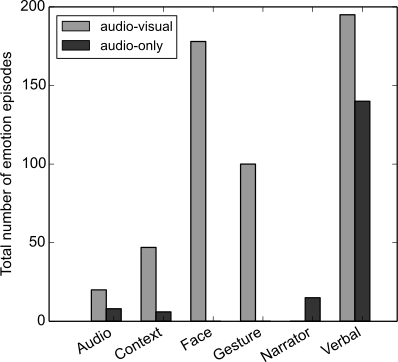
\includegraphics[trim=00 40 35 26,clip,width=\linewidth]{figures/labeledoncue_episodes}
  \caption{Number of emotion episodes for all distinguished onset cue categories
    (minimum \AVAggThresh\ inter-rater agreement) for both stimulus types.}
  \label{fig:threshlabeledoncue}
\end{figure}

\subsection*{Observer agreement as a probabilistic indicator}

It can be assumed that observers in this study have used individual intensity
thresholds for determining the start, end, or quality of an emotional episode.
Therefore, the IOA with respect to a particular aspect of portrayed emotions at
any given time in the movie could be seen as a measure of the relative
probability of perceiving an emotion feature. In order to assess the
reliability of such a measure, we generated time series for the IOA with a
sampling rate of \unit[1]{Hz}, as described above, and evaluated their
reliability and validity in terms of their correlation across observers,
stimulus types, and with each other.

\begin{figure*}
  \centering
  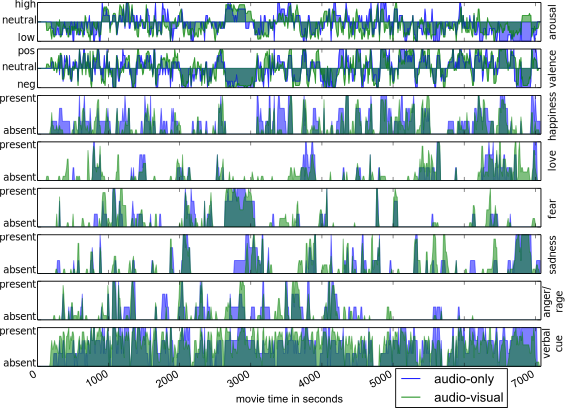
\includegraphics[trim=10 75 70 50,clip,width=\linewidth]{figures/indicator_ts_allchar}\\
  %includegraphics[width=\linewidth]{figures/indicator_ts_forrest}
  \caption{Inter-observer agreement (IOA) time courses for selected emotion
    attributes across the full duration of the movie. Extreme values indicate
    perfect agreement with respect to presence or absence of a particular emotion
    attribute at a given time. IOA time series for the two movie types are
    overlayed on top of each other.
    For the purpose of
    visualization, the depicted time series reflects IOA computed using a
    \unit[10]{s} segment size --- in contrast to \unit[1]{s} used for all other
  statistics presented in this paper.}
  \label{fig:indicatortsallchar}
\end{figure*}


\paragraph{Intra-stimulus inter-observer consistency}

The reliability of IOA time courses was estimated by repeatedly splitting the
set of observers into two groups of approximately equal size. Within each
group, IOA time courses where computed and correlated across the observer
sub-groups. Split-half correlations were computed for all possible ways of
combining observers into two groups (without replacement).
Table~\ref{tab:interobserver_consistency} shows the average time series
correlation across all splits and the width of the 95\% confidence interval of
the mean.

In general, IOA reliability is larger for the AV movie annotations than for the
AO movie. This finding is likely a result of the lower number of observers for
the latter. Intra-stimulus IOA reliability estimates suggest that a subset of
emotion attributes or categories is not contained in the AO movie stimulus.
The most prominent example is the direction of an emotion. Emotion categories
like hate, shame, or relief also show large reliability differences between
stimulus types. However, in these cases the small number of emotion episodes
may multiply the negative effect of the small number of observers on the
interpretability of this estimate.

Uniformly high reliability estimates were found for the two main dimensional
emotion attributes arousal and valence, as well as for the five most frequently
annotated emotion categories anger/rage, fear, happiness, love, and sadness.

\begin{table*}
  \centering
  \begin{tabular}{p{18mm}cccccc}
    & \multicolumn{2}{c}{\textbf{All characters}} & \multicolumn{2}{c}{\textbf{Forrest-only}} & \multicolumn{2}{c}{\textbf{Jenny-only}} \\
    & \textbf{Audio-visual} & \textbf{Audio-only} & \textbf{Audio-visual} & \textbf{Audio-only} & \textbf{Audio-visual} & \textbf{Audio-only} \\
    \\\hline\\
    \multicolumn{7}{l}{\textit{Dimensional emotion attributes}}\\
    Arousal & \AVInterRaterConsistArousalAllChar & \AOInterRaterConsistArousalAllChar & \AVInterRaterConsistArousalForrest & \AOInterRaterConsistArousalForrest & \AVInterRaterConsistArousalJenny & \AOInterRaterConsistArousalJenny \\
    Valence & \AVInterRaterConsistValenceAllChar & \AOInterRaterConsistValenceAllChar & \AVInterRaterConsistValenceForrest & \AOInterRaterConsistValenceForrest & \AVInterRaterConsistValenceJenny & \AOInterRaterConsistValenceJenny \\
    Direction & \AVInterRaterConsistDirectionAllChar & \AOInterRaterConsistDirectionAllChar & \AVInterRaterConsistDirectionForrest & \AOInterRaterConsistDirectionForrest & \AVInterRaterConsistDirectionJenny & \AOInterRaterConsistDirectionJenny \\
    \\\hline\\

    \multicolumn{7}{l}{\textit{Emotion categories}}\\
    Admiration     & \AVInterRaterConsistADMIRATIONAllChar     & \AOInterRaterConsistADMIRATIONAllChar     &\AVInterRaterConsistADMIRATIONForrest     &\AOInterRaterConsistADMIRATIONForrest     &\AVInterRaterConsistADMIRATIONJenny     &\AOInterRaterConsistADMIRATIONJenny     \\
    Anger/Rage     & \AVInterRaterConsistANGERRAGEAllChar      & \AOInterRaterConsistANGERRAGEAllChar      &\AVInterRaterConsistANGERRAGEForrest      &\AOInterRaterConsistANGERRAGEForrest      &\AVInterRaterConsistANGERRAGEJenny      &\AOInterRaterConsistANGERRAGEJenny      \\
    Compassion     & \AVInterRaterConsistCOMPASSIONAllChar     & \AOInterRaterConsistCOMPASSIONAllChar     &\AVInterRaterConsistCOMPASSIONForrest     &\AOInterRaterConsistCOMPASSIONForrest     &\AVInterRaterConsistCOMPASSIONJenny     &\AOInterRaterConsistCOMPASSIONJenny     \\
    Contempt       & \AVInterRaterConsistCONTEMPTAllChar       & \AOInterRaterConsistCONTEMPTAllChar       &\AVInterRaterConsistCONTEMPTForrest       &\AOInterRaterConsistCONTEMPTForrest       &\AVInterRaterConsistCONTEMPTJenny       &\AOInterRaterConsistCONTEMPTJenny       \\
    Disappoint. & \AVInterRaterConsistDISAPPOINTMENTAllChar & \AOInterRaterConsistDISAPPOINTMENTAllChar &\AVInterRaterConsistDISAPPOINTMENTForrest &\AOInterRaterConsistDISAPPOINTMENTForrest &\AVInterRaterConsistDISAPPOINTMENTJenny &\AOInterRaterConsistDISAPPOINTMENTJenny \\
    Fear           & \AVInterRaterConsistFEARAllChar           & \AOInterRaterConsistFEARAllChar           &\AVInterRaterConsistFEARForrest           &\AOInterRaterConsistFEARForrest           &\AVInterRaterConsistFEARJenny           &\AOInterRaterConsistFEARJenny           \\
    Fears conf.          & \AVInterRaterConsistFEARSCONFIRMEDAllChar           & \AOInterRaterConsistFEARSCONFIRMEDAllChar           &\AVInterRaterConsistFEARSCONFIRMEDForrest           &\AOInterRaterConsistFEARSCONFIRMEDForrest           &\AVInterRaterConsistFEARSCONFIRMEDJenny           &\AOInterRaterConsistFEARSCONFIRMEDJenny           \\
    Gloating       & \AVInterRaterConsistGLOATINGAllChar       & \AOInterRaterConsistGLOATINGAllChar       &\AVInterRaterConsistGLOATINGForrest       &\AOInterRaterConsistGLOATINGForrest       &\AVInterRaterConsistGLOATINGJenny       &\AOInterRaterConsistGLOATINGJenny       \\
    Gratification  & \AVInterRaterConsistGRATIFICATIONAllChar  & \AOInterRaterConsistGRATIFICATIONAllChar  &\AVInterRaterConsistGRATIFICATIONForrest  &\AOInterRaterConsistGRATIFICATIONForrest  &\AVInterRaterConsistGRATIFICATIONJenny  &\AOInterRaterConsistGRATIFICATIONJenny  \\
    Gratitude      & \AVInterRaterConsistGRATITUDEAllChar      & \AOInterRaterConsistGRATITUDEAllChar      &\AVInterRaterConsistGRATITUDEForrest      &\AOInterRaterConsistGRATITUDEForrest      &\AVInterRaterConsistGRATITUDEJenny      &\AOInterRaterConsistGRATITUDEJenny      \\
    Happiness      & \AVInterRaterConsistHAPPINESSAllChar      & \AOInterRaterConsistHAPPINESSAllChar      &\AVInterRaterConsistHAPPINESSForrest      &\AOInterRaterConsistHAPPINESSForrest      &\AVInterRaterConsistHAPPINESSJenny      &\AOInterRaterConsistHAPPINESSJenny      \\
    Happy-for      & \AVInterRaterConsistHAPPYFORAllChar       & \AOInterRaterConsistHAPPYFORAllChar       &\AVInterRaterConsistHAPPYFORForrest       &\AOInterRaterConsistHAPPYFORForrest       &\AVInterRaterConsistHAPPYFORJenny       &\AOInterRaterConsistHAPPYFORJenny       \\
    Hate           & \AVInterRaterConsistHATEAllChar           & \AOInterRaterConsistHATEAllChar           &\AVInterRaterConsistHATEForrest           &\AOInterRaterConsistHATEForrest           &\AVInterRaterConsistHATEJenny           &\AOInterRaterConsistHATEJenny           \\
    Hope           & \AVInterRaterConsistHOPEAllChar           & \AOInterRaterConsistHOPEAllChar           &\AVInterRaterConsistHOPEForrest           &\AOInterRaterConsistHOPEForrest           &\AVInterRaterConsistHOPEJenny           &\AOInterRaterConsistHOPEJenny           \\
    Love           & \AVInterRaterConsistLOVEAllChar           & \AOInterRaterConsistLOVEAllChar           &\AVInterRaterConsistLOVEForrest           &\AOInterRaterConsistLOVEForrest           &\AVInterRaterConsistLOVEJenny           &\AOInterRaterConsistLOVEJenny           \\
    Pride          & \AVInterRaterConsistPRIDEAllChar          & \AOInterRaterConsistPRIDEAllChar          &\AVInterRaterConsistPRIDEForrest          &\AOInterRaterConsistPRIDEForrest          &\AVInterRaterConsistPRIDEJenny          &\AOInterRaterConsistPRIDEJenny          \\
    Relief         & \AVInterRaterConsistRELIEFAllChar         & \AOInterRaterConsistRELIEFAllChar         &\AVInterRaterConsistRELIEFForrest         &\AOInterRaterConsistRELIEFForrest         &\AVInterRaterConsistRELIEFJenny         &\AOInterRaterConsistRELIEFJenny         \\
    Remorse        & \AVInterRaterConsistREMORSEAllChar        & \AOInterRaterConsistREMORSEAllChar        &\AVInterRaterConsistREMORSEForrest        &\AOInterRaterConsistREMORSEForrest        &\AVInterRaterConsistREMORSEJenny        &\AOInterRaterConsistREMORSEJenny        \\
    Resentment     & \AVInterRaterConsistRESENTMENTAllChar     & \AOInterRaterConsistRESENTMENTAllChar     &\AVInterRaterConsistRESENTMENTForrest     &\AOInterRaterConsistRESENTMENTForrest     &\AVInterRaterConsistRESENTMENTJenny     &\AOInterRaterConsistRESENTMENTJenny     \\
    Sadness        & \AVInterRaterConsistSADNESSAllChar        & \AOInterRaterConsistSADNESSAllChar        &\AVInterRaterConsistSADNESSForrest        &\AOInterRaterConsistSADNESSForrest        &\AVInterRaterConsistSADNESSJenny        &\AOInterRaterConsistSADNESSJenny        \\
    Satisfaction   & \AVInterRaterConsistSATISFACTIONAllChar   & \AOInterRaterConsistSATISFACTIONAllChar   &\AVInterRaterConsistSATISFACTIONForrest   &\AOInterRaterConsistSATISFACTIONForrest   &\AVInterRaterConsistSATISFACTIONJenny   &\AOInterRaterConsistSATISFACTIONJenny   \\
    Shame          & \AVInterRaterConsistSHAMEAllChar          & \AOInterRaterConsistSHAMEAllChar          &\AVInterRaterConsistSHAMEForrest          &\AOInterRaterConsistSHAMEForrest          &\AVInterRaterConsistSHAMEJenny          &\AOInterRaterConsistSHAMEJenny          \\\\                  
    \hline\\
    \multicolumn{7}{l}{\textit{Emotion onset cues}}\\
    Audio & \AVInterRaterConsistAUDIOAllChar &\AOInterRaterConsistAUDIOAllChar &\AVInterRaterConsistAUDIOForrest &\AOInterRaterConsistAUDIOForrest &\AVInterRaterConsistAUDIOJenny &\AOInterRaterConsistAUDIOJenny \\
    Context & \AVInterRaterConsistCONTEXTAllChar & \AOInterRaterConsistCONTEXTAllChar &\AVInterRaterConsistCONTEXTForrest &\AOInterRaterConsistCONTEXTForrest &\AVInterRaterConsistCONTEXTJenny &\AOInterRaterConsistCONTEXTJenny \\
    Face & \AVInterRaterConsistFACEAllChar & \AOInterRaterConsistFACEAllChar &\AVInterRaterConsistFACEForrest &\AOInterRaterConsistFACEForrest &\AVInterRaterConsistFACEJenny &\AOInterRaterConsistFACEJenny \\
    Gesture & \AVInterRaterConsistGESTUREAllChar & \AOInterRaterConsistGESTUREAllChar &\AVInterRaterConsistGESTUREForrest &\AOInterRaterConsistGESTUREForrest &\AVInterRaterConsistGESTUREJenny &\AOInterRaterConsistGESTUREJenny \\
    Narrator & \AVInterRaterConsistNARRATORAllChar & \AOInterRaterConsistNARRATORAllChar &\AVInterRaterConsistNARRATORForrest  &\AOInterRaterConsistNARRATORForrest &\AVInterRaterConsistNARRATORJenny &\AOInterRaterConsistNARRATORJenny \\
    Verbal & \AVInterRaterConsistVERBALAllChar & \AOInterRaterConsistVERBALAllChar &\AVInterRaterConsistVERBALForrest  &\AOInterRaterConsistVERBALForrest &\AVInterRaterConsistVERBALJenny &\AOInterRaterConsistVERBALJenny \\
    \\\hline


%    \multicolumn{7}{l}{\textit{Intra-stimulus indicator correlation}} \\\\
%    Arousal-Valence & \AVCorrArousalValenceAllChar & \AOCorrArousalValenceAllChar & \AVCorrArousalValenceForrest & \AOCorrArousalValenceForrest & \AVCorrArousalValenceJenny & \AOCorrArousalValenceJenny \\
%    Arousal-Direction & \AVCorrArousalDirectionAllChar & \AOCorrArousalDirectionAllChar & \AVCorrArousalDirectionForrest & \AOCorrArousalDirectionForrest & \AVCorrArousalDirectionJenny & \AOCorrArousalDirectionJenny \\
%    Valence-Direction & \AVCorrValenceDirectionAllChar & \AOCorrValenceDirectionAllChar & \AVCorrValenceDirectionForrest & \AOCorrValenceDirectionForrest & \AVCorrValenceDirectionJenny & \AOCorrValenceDirectionJenny \\
%    \\\hline\\
  \end{tabular}

  \caption{
    Intra-stimulus inter-observer consistency. All values are Spearman
    correlations for \unit[1]{Hz} modulations of the fraction of
    IOA (as, for example, depicted in figure
    \ref{fig:indicatortsallchar}) with respect to a particular emotion
    attribute across the entire duration of the movie. The specified range
    corresponds to the width of the 95\% confidence interval of the mean correlation
    for all possible combinations of partitioning observers into two sub-groups (audio-visual
    4~vs.~5; audio-only 1~vs~2). Higher correlations indicate higher consistency
    of agreement modulations across observer sub-groups.
    The \textit{all characters} column indicates the agreement for a particular
    emotion attribute over time irrespective of the annotated character. The
    columns on the right show the corresponding correlations for the two main
    characters. \textit{n/a} fields indicate an insufficient number of annotations to compute
    the consistency measure.}
  \label{tab:interobserver_consistency}
\end{table*}

\paragraph{Intra-stimulus inter-variable correlations}

In order to assess possible confounds in the annotations, we computed the
correlation of intra-stimulus IOA time courses (across all observers) for all
pairwise combinations of emotion attributes and categories. The correlation
matrices for the AV and the AO movie stimulus are depicted in figure
\ref{fig:intrastimcorrelation}. The results reveal an expected correlation
pattern between individual emotion categories and the two main dimensional
attributes arousal and valence --- with stronger correlations being observed for
more primary and more frequently portrayed emotions. Interestingly, audio and
verbal cues in the AV stimulus seems to be more associated with a high state of
arousal and emotions directed towards other people than in the AO stimulus. In
the AV stimulus, facial expressions seem to have a tendency to communicate
negative emotions rather than positive ones.


\begin{figure*}
  \centering
  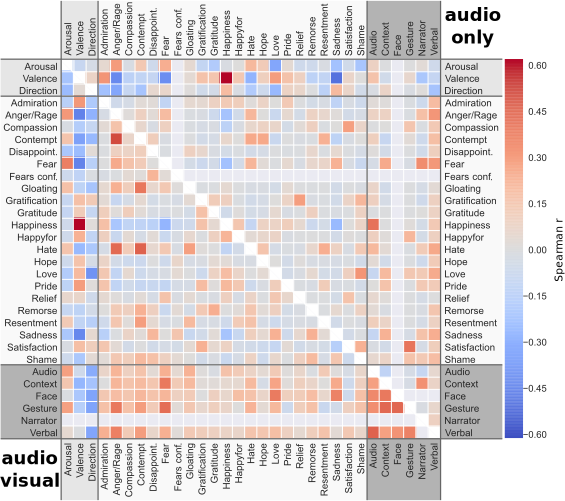
\includegraphics[width=\linewidth]{figures/bigcorr}
  \caption{Intra-stimulus indicator correlation. The lower triangular matrix
    depicts the correlations between the IOA time courses for
    the three primary bipolar emotion attributes (arousal [high/low], valence [pos/neg], and direction [self/other]), the
    22 emotion categories, and the six emotion onset indicators for the audio-visual
    movie. The upper triangular matrix shows the corresponding correlations for the
    audio-only movie.
 }
  \label{fig:intrastimcorrelation}
\end{figure*}

\paragraph{Inter-stimulus consistency}

To estimate the similarity of the two stimulus types, we computed the
correlation of IOA time courses for the AV and the AO movie with respective to
emotion attributes and categories. Table~\ref{tab:interstim_consistency} shows
the respective correlations and their 95\% confidence interval. Again, the
three dimensional attributes as well as the five most frequent emotion
categories show significant correlations. This is evidence for an expected
substantial semantic similarity with respected to the emotional content in the
two variants of the ``Forrest Gump'' movie.

\begin{table*}
  \centering
  \begin{tabular}{p{26mm}ccc}
    & \textbf{All characters} & \textbf{Forrest-only} & \textbf{Jenny-only} \\
    \hline \\
    \multicolumn{4}{l}{\textit{Dimensional emotion attributes}}\\
    Arousal & \InterModCorrArousalAllChar &\InterModCorrArousalForrest &\InterModCorrArousalJenny \\
    Valence & \InterModCorrValenceAllChar &\InterModCorrValenceForrest &\InterModCorrValenceJenny \\
    Direction & \InterModCorrDirectionAllChar &\InterModCorrDirectionForrest &\InterModCorrDirectionJenny \\\\\hline\\

    \multicolumn{4}{l}{\textit{Emotion categories}}\\
    Admiration & \InterModCorrADMIRATIONAllChar &\InterModCorrADMIRATIONForrest &\InterModCorrADMIRATIONJenny \\
    Anger/Rage & \InterModCorrANGERRAGEAllChar &\InterModCorrANGERRAGEForrest &\InterModCorrANGERRAGEJenny \\
    Compassion & \InterModCorrCOMPASSIONAllChar &\InterModCorrCOMPASSIONForrest &\InterModCorrCOMPASSIONJenny \\
    Contempt & \InterModCorrCONTEMPTAllChar &\InterModCorrCONTEMPTForrest &\InterModCorrCONTEMPTJenny \\
    Disappointment & \InterModCorrDISAPPOINTMENTAllChar &\InterModCorrDISAPPOINTMENTForrest &\InterModCorrDISAPPOINTMENTJenny \\
    Fear & \InterModCorrFEARAllChar &\InterModCorrFEARForrest &\InterModCorrFEARJenny \\
    Gloating & \InterModCorrGLOATINGAllChar &\InterModCorrGLOATINGForrest &\InterModCorrGLOATINGJenny \\
    Gratification & \InterModCorrGRATIFICATIONAllChar &\InterModCorrGRATIFICATIONForrest &\InterModCorrGRATIFICATIONJenny \\
    Gratitude & \InterModCorrGRATITUDEAllChar &\InterModCorrGRATITUDEForrest &\InterModCorrGRATITUDEJenny \\
    Happiness & \InterModCorrHAPPINESSAllChar &\InterModCorrHAPPINESSForrest &\InterModCorrHAPPINESSJenny \\
    Happy-for & \InterModCorrHAPPYFORAllChar &\InterModCorrHAPPYFORForrest &\InterModCorrHAPPYFORJenny \\
    Hate & \InterModCorrHATEAllChar &\InterModCorrHATEForrest &\InterModCorrHATEJenny \\
    Hope & \InterModCorrHOPEAllChar &\InterModCorrHOPEForrest &\InterModCorrHOPEJenny \\
    Love & \InterModCorrLOVEAllChar &\InterModCorrLOVEForrest &\InterModCorrLOVEJenny \\
    Pride & \InterModCorrPRIDEAllChar &\InterModCorrPRIDEForrest &\InterModCorrPRIDEJenny \\
    Relief & \InterModCorrRELIEFAllChar &\InterModCorrRELIEFForrest &\InterModCorrRELIEFJenny \\
    Remorse & \InterModCorrREMORSEAllChar &\InterModCorrREMORSEForrest &\InterModCorrREMORSEJenny \\
    Resentment & \InterModCorrRESENTMENTAllChar &\InterModCorrRESENTMENTForrest &\InterModCorrRESENTMENTJenny \\
    Sadness & \InterModCorrSADNESSAllChar &\InterModCorrSADNESSForrest &\InterModCorrSADNESSJenny \\
    Satisfaction & \InterModCorrSATISFACTIONAllChar &\InterModCorrSATISFACTIONForrest &\InterModCorrSATISFACTIONJenny \\
    Shame & \InterModCorrSHAMEAllChar &\InterModCorrSHAMEForrest &\InterModCorrSHAMEJenny \\
    \\\hline\\
    \multicolumn{4}{l}{\textit{Emotion onset cues}}\\
    Audio & \InterModCorrAUDIOAllChar &\InterModCorrAUDIOForrest &\InterModCorrAUDIOJenny \\
    Context & \InterModCorrCONTEXTAllChar &\InterModCorrCONTEXTForrest &\InterModCorrCONTEXTJenny \\
    %Face & \InterModCorrFACEAllChar &\InterModCorrFACEForrest &\InterModCorrFACEJenny \\
    %Gesture & \InterModCorrGESTUREAllChar &\InterModCorrGESTUREForrest &\InterModCorrGESTUREJenny \\
    %Narrator & \InterModCorrNARRATORAllChar &\InterModCorrNARRATORForrest &\InterModCorrNARRATORJenny \\
    Verbal & \InterModCorrVERBALAllChar &\InterModCorrVERBALForrest &\InterModCorrVERBALJenny \\
    \\\hline

  \end{tabular}

  \caption{ Inter-stimulus indicator correlation. All values are Spearman
    correlations of \unit[1]{Hz} modulations of the fraction of
    IOA (as, for example, depicted in figure
    \ref{fig:indicatortsallchar}) for the two stimulus types (audio-visual and
  audio-only movie). The specified range corresponds to the width of the 95\%
confidence interval of the correlation (computed via Fisher
transformation).}


  \label{tab:interstim_consistency}
\end{table*}

\hl{TODO: are there annotations that do not contain indicators specifications?

Current: \AVFracWithLabeledOncue \AOFracWithLabeledOncue
}


\section*{Data availability}

\texttt{This section will be auto-generated.}


\section*{Author contributions}
%In order to give appropriate credit to each author of an article, the
%individual contributions of each author to the manuscript should be detailed
%in this section. We recommend using author initials and then stating briefly
%how they contributed.
AKP, AL, BH, FRS, HS, LNR, MB, MGE, MGO, MP, NH, SK, and TR designed the data
collection procedure, performed the annotation, and contributed to the
manuscript; MH conceived the study, aggregated data from individual observers
into the released form, performed the data analysis, and contributed to the
manuscript.
%MK; LG;

\section*{Competing Interests}
No competing interests were disclosed.

\section*{Grant Information}

This research was, in part, supported by the German Federal Ministry of
Education and Research (BMBF) as part of a US-German collaboration in
computational neuroscience (CRCNS; awarded to James Haxby, Peter Ramadge, and
Michael Hanke), co-funded by the BMBF and the US National Science Foundation
(BMBF 01GQ1112; NSF 1129855). Michael Hanke was supported by funds from the
German federal state of Saxony-Anhalt, Project: Center for Behavioral Brain
Sciences.

\section*{Acknowledgements}
%This section should acknowledge anyone who contributed to the research or the
%article but who does not qualify as an author based on the criteria provided
%earlier (e.g. someone or an organisation that provided writing assistance).
%Please state how they contributed; authors should obtain permission to
%acknowledge from all those mentioned in the Acknowledgements section.  Please
%do not list grant funding in this section (this should be included in the
%Grant information section - See above).

We are grateful to Roland Nigbur for his advice during all stages of this
study and for his feedback on the manuscript.

%\nocite{*}
{\small\bibliographystyle{unsrt}
\bibliography{bibliography/biblio}}

\end{document}

% vim: textwidth=80 colorcolumn=81
